%! TeX program = lualatex
\documentclass[12pt, fleqn]{extarticle}
\usepackage[english,russian]{babel}
\usepackage{fontspec}
\usepackage{graphicx}
\usepackage{indentfirst}
\usepackage{caption}
\usepackage{wrapfig}
\usepackage{amsmath}
\usepackage{hyperref}
\usepackage{enumitem} % no item sep in list
\usepackage[explicit]{titlesec}
% \usepackage{geometry}
% \usepackage{emoji}
% \usepackage{amsmath}
% \usepackage{xcolor, cancel}
% \usepackage{stackengine}
% \usepackage{ulem}
% \usepackage{amsthm}
% \usepackage{tikz}
% \usepackage{multicol}
% \usepackage{pgfplots}
% \usepackage{ragged2e}
% \usepackage{xifthen}
% \usepackage{amssymb}
% \usepackage{unicode-math}

\setmainfont{PT Serif}

\titleformat{\section}
{\Large}{\textbf{\thesection.}}{0.5em}{\textbf{#1}} \usepackage{textcomp}

\usepackage[%
    left=1.25in,%
    right=1.25in,%
    top=1.1in,%
    bottom=1.1in,%
]{geometry}%

\hypersetup{
    colorlinks=true,
    linkcolor=black,
    filecolor=magenta,
    urlcolor=cyan,
    pdftitle={Ответы на билеты по математике 2021},
    pdfpagemode=FullScreen,
}

\captionsetup[figure]{labelformat=empty, labelsep=none}
\graphicspath{ {./images/} }

\begin{document}

\section*{Быстрое перемещение}

Для перемещения \textbf{нажмите} на название требуемого раздела:
\begin{enumerate}[noitemsep]
    \item \hyperref[sec:linear-dependence]{Линейная зависимость системы векторов. Базис}
    \item \hyperref[sec:det]{Свойства определителей}
    \item \hyperref[sec:line]{Прямая на плоскости: уравнение через две точки, каноническое, параметрическое, общее}
    \item \hyperref[sec:parabola]{Парабола. Определение, вывод уравнения, характеристики}
\end{enumerate}

\newpage

\section{Линейная зависимость системы векторов. \\ Базис}\label{sec:linear-dependence}

\subsection*{Определения}

\subsubsection*{Линейная комбинация}
Линейной комбинацией \(n\) векторов \(\overrightarrow{a_1}, \overrightarrow{a_2}, ..., \overrightarrow{a_n}\) называется сумма произведений этих векторов на произвольные вещественные числа, то есть выражения вида:
\begin{align*}
     &  &
    \lambda_1 \cdot \overrightarrow{a_1} + \lambda_2 \overrightarrow{a_2} + ... + \lambda_n + \overrightarrow{a_n}
\end{align*}

где \(\lambda_1, \lambda_2, ..., \lambda_n\) — любые действительные числа.

\subsubsection*{Линейно зависимая система векторов}
Если для линейная комбинация \(\lambda_1 \cdot \overrightarrow{a_1} + \lambda_2 \cdot \overrightarrow{a_2} + ... + \lambda_n \cdot \overrightarrow{a_n}\) равна нулевому вектору (нулю) при условии, что хотя бы одно из чисел \(\lambda_1, \lambda_2, ..., \lambda_n\) отлично от нуля, то система векторов \(\overrightarrow{a_1}, \overrightarrow{a_2}, ..., \overrightarrow{a_n}\) называется \textbf{линейно зависимой}.

\subsubsection*{Линейно \underline{не}зависимая система векторов}
Если для линейная комбинация \(\lambda_1 \cdot \overrightarrow{a_1} + \lambda_2 \cdot \overrightarrow{a_2} + ... + \lambda_n \cdot \overrightarrow{a_n}\) равна нулевому вектору (нулю) \textbf{только тогда}, когда все числа \(\lambda_1, \lambda_2, ..., \lambda_n\) равны нулю, то система векторов \(\overrightarrow{a_1}, \overrightarrow{a_2}, ..., \overrightarrow{a_n}\) называется \textbf{линейно независимой}.

\subsection*{Свойства линейной зависимости и независимости}

1. Если к линейно зависимой системе векторов \(\overrightarrow{a_1}, \overrightarrow{a_2}, ..., \overrightarrow{a_n}\) добавить несколько векторов, то полученная система будет линейно \textbf{зависимой}.

2. Если из линейно независимой системы векторов \(\overrightarrow{a_1}, \overrightarrow{a_2}, ..., \overrightarrow{a_n}\) исключить несколько векторов, то полученная система будет линейно \textbf{независимой}.

3. Если в системе векторов \(\overrightarrow{a_1}, \overrightarrow{a_2}, ..., \overrightarrow{a_n}\) есть хотя бы один нулевой вектор, то такая система линейно зависимая.

4. Если система векторов \(\overrightarrow{a_1}, \overrightarrow{a_2}, ..., \overrightarrow{a_n}\) линейно зависима, то хотя бы один из ее векторов линейно выражается через остальные. Если система векторов линейно независима, то ни один из векторов не выражается через остальные.

Из двух последних свойств следует важное утверждение:
если система векторов содержит векторы \(\overrightarrow{a}\) и \(c \overrightarrow{a}\), где \(c\) – произвольное число, то она линейно зависима.

\subsection*{Размерность и базис}
\textbf{Размерностью векторного пространства} называется число, равное максимальному количеству линейно \textbf{независимых} векторов в этом пространстве.

\textbf{Базис векторного пространства} – это упорядоченная совокупность линейно \textbf{независимых} векторов этого пространства, число которых равно размерности пространства.

\newpage

\section{Скалярное произведение векторов и его свойства. Проекции}

Скалярное произведение векторов \(\overrightarrow{a}\) и \(\overrightarrow{b}\) есть ничто иное как:
\begin{align*}
     &  &
    (\overrightarrow{a}, \overrightarrow{b}) = |\overrightarrow{a}| \cdot |\overrightarrow{b}| \cdot \cos{\varphi},
\end{align*}

где \(\varphi\) — величина угла между векторами \(\overrightarrow{a}\) и \(\overrightarrow{b}\).

\subsection*{Свойства скалярного произведения}

\begin{enumerate}[noitemsep]
    \item \((\overrightarrow{a}, \overrightarrow{b}) = (\overrightarrow{b}, \overrightarrow{a})\)

    \item \((\overrightarrow{a} + \overrightarrow{b}, \overrightarrow{c}) = (\overrightarrow{a}, \overrightarrow{c}) + (\overrightarrow{b} + \overrightarrow{c})\)

    \item \((\lambda \cdot \overrightarrow{a}, \overrightarrow{b}) = \lambda \cdot (\overrightarrow{a}, \overrightarrow{b})\), где \(\lambda \in R\).

    \item \((\overrightarrow{a}, \overrightarrow{a}) \geq 0\), причем \((\overrightarrow{a}, \overrightarrow{a}) = 0 \iff |\overrightarrow{a}| = 0\)

    \item \(\overrightarrow{a}^2 = |\overrightarrow{a}|^2\)

    \item \(\cos{\varphi} = \dfrac{(\overrightarrow{a}, \overrightarrow{b})}{|\overrightarrow{a}| \cdot |\overrightarrow{b}|}\), где \(\varphi\) угол между векторами \(\overrightarrow{a}\) и \(\overrightarrow{b}\).

    \item \(\overrightarrow{a} \perp \overrightarrow{b} \iff (\overrightarrow{a}, \overrightarrow{b}) = 0\)

    \item Угол между двумя ненулевыми векторами \(\overrightarrow{a}\) и \(\overrightarrow{b}\) является острым тогда и только тогда, когда \((\overrightarrow{a}, \overrightarrow{b}) > 0\); и является тупым – когда \((\overrightarrow{a}, \overrightarrow{b}) < 0\).

    \item \(\text{Пр}_{b}\overrightarrow{a} = \dfrac{(\overrightarrow{a}, \overrightarrow{b})}{|\overrightarrow{b}|}\)
\end{enumerate}


\newpage

\section{Свойства определителей}\label{sec:det}

1. Определитель транспонированной матрицы равен определителю исходной матрицы: \(\det A^T = \det A\)

2. Умножение всех элементов строки или столбца определителя на некоторое число \lambda равносильно умножееию определителя на это число:
\begin{align*}
     &  &
    \begin{vmatrix}
        a_{11}         & a_{12}         & \dots a_{1j}         & \dots & a_{1n}         \\
        a_{21}         & a_{22}         & \dots a_{2j}         & \dots & a_{2n}         \\
        \dots          & \dots          & \dots                & \dots & \dots          \\
        \lambda a_{i1} & \lambda a_{i2} & \dots \lambda a_{ij} & \dots & \lambda a_{in} \\
        \dots          & \dots          & \dots                & \dots & \dots          \\
        a_{m1}         & a_{m2}         & \dots a_{mj}         & \dots & a_{mn}         \\
    \end{vmatrix}
    =
    \lambda \cdot
    \begin{vmatrix}
        a_{11} & a_{12} & \dots a_{1j} & \dots & a_{1n} \\
        a_{21} & a_{22} & \dots a_{2j} & \dots & a_{2n} \\
        \dots  & \dots  & \dots        & \dots & \dots  \\
        a_{i1} & a_{i2} & \dots a_{ij} & \dots & a_{in} \\
        \dots  & \dots  & \dots        & \dots & \dots  \\
        a_{m1} & a_{m2} & \dots a_{mj} & \dots & a_{mn} \\
    \end{vmatrix}
\end{align*}

3. Если в определителе переставить местами любые две строки или два столбца, то определитель изменяет свой знак на противоположный:
\begin{align*}
     &  &
    \begin{vmatrix}
        \dots  & \dots  & \dots  & \dots & \dots  \\
        a_{i1} & a_{i2} & a_{i3} & \dots & a_{in} \\
        \dots  & \dots  & \dots  & \dots & \dots  \\
        a_{k1} & a_{k2} & a_{k3} & \dots & a_{kn} \\
        \dots  & \dots  & \dots  & \dots & \dots  \\
    \end{vmatrix}
    =
    -
    \begin{vmatrix}
        \dots  & \dots  & \dots  & \dots & \dots  \\
        a_{k1} & a_{k2} & a_{k3} & \dots & a_{kn} \\
        \dots  & \dots  & \dots  & \dots & \dots  \\
        a_{i1} & a_{i2} & a_{i3} & \dots & a_{in} \\
        \dots  & \dots  & \dots  & \dots & \dots  \\
    \end{vmatrix}
\end{align*}

4. Если матрица содержит нулевую строку (столбец), то определитель этой матрицы равен нулю:
\begin{align*}
     &  &
    \begin{vmatrix}
        \dots  & \dots  & \dots  & \dots & \dots  \\
        a_{i1} & a_{i2} & a_{i3} & \dots & a_{in} \\
        0      & 0      & 0      & \dots & 0      \\
        a_{j1} & a_{j2} & a_{j3} & \dots & a_{jn} \\
        \dots  & \dots  & \dots  & \dots & \dots  \\
    \end{vmatrix}
    = 0
\end{align*}

5. Если две строки (столбца) матрицы равны между собой, то определитель этой матрицы равен нулю:
\begin{align*}
     &  &
    \begin{vmatrix}
        \dots  & \dots  & \dots  & \dots & \dots  \\
        a_{i1} & a_{i2} & a_{i3} & \dots & a_{in} \\
        \dots  & \dots  & \dots  & \dots & \dots  \\
        a_{i1} & a_{i2} & a_{i3} & \dots & a_{in} \\
        \dots  & \dots  & \dots  & \dots & \dots  \\
    \end{vmatrix}
    = 0
\end{align*}

6. Если две строки (столбца) матрицы пропорциональны друг другу, то определитель этой матрицы равен нулю:
\begin{align*}
     &  &
    \begin{vmatrix}
        \dots   & \dots   & \dots   & \dots & \dots   \\
        a_{i1}  & a_{i2}  & a_{i3}  & \dots & a_{in}  \\
        \dots   & \dots   & \dots   & \dots & \dots   \\
        ca_{i1} & ca_{i2} & ca_{i3} & \dots & ca_{in} \\
        \dots   & \dots   & \dots   & \dots & \dots   \\
    \end{vmatrix}
    = 0
\end{align*}

7. Определитель матрицы треугольного вида равен произведению элементов, стоящих на главной диагонали:
\begin{align*}
     &  &
    \begin{vmatrix}
        a_{11} & a_{12} & a_{13} & \dots & a_{1n} \\
        0      & a_{22} & a_{23} & \dots & a_{2n} \\
        0      & 0      & a_{33} & \dots & a_{3n} \\
        \dots  & \dots  & \dots  & \dots & \dots  \\
        0      & 0      & 0      & \dots & a_{mn} \\
    \end{vmatrix}
    = a_{11} \cdot a_{22} \cdot a_{33} \cdot ... \cdot a_{mn}
\end{align*}

8. Если все элементы k-ой строки (столбца) определителя представлены в виде сумм \(a_{kj} + b_{kj}\), то определитель можно представить в виде суммы соответствующих определителей:
\begin{align*}
     &  &
    \begin{vmatrix}
        a_{11}          & a_{12}          & a_{13}          & \dots & a_{1n}          \\
        \dots           & \dots           & \dots           & \dots & \dots           \\
        a_{k1} + b_{k1} & a_{k2} + b_{k2} & a_{k3} + b_{k3} & \dots & a_{kn} + b_{kn} \\
        \dots           & \dots           & \dots           & \dots & \dots           \\
        a_{m1}          & a_{m2}          & a_{m3}          & \dots & a_{mn}          \\
    \end{vmatrix}
    =
    \\
     &  &
    =
    \begin{vmatrix}
        a_{11} & a_{12} & a_{13} & \dots & a_{1n} \\
        \dots  & \dots  & \dots  & \dots & \dots  \\
        a_{k1} & a_{k2} & a_{k3} & \dots & a_{kn} \\
        \dots  & \dots  & \dots  & \dots & \dots  \\
        a_{m1} & a_{m2} & a_{m3} & \dots & a_{mn} \\
    \end{vmatrix}
    +
    \begin{vmatrix}
        a_{11} & a_{12} & a_{13} & \dots & a_{1n} \\
        \dots  & \dots  & \dots  & \dots & \dots  \\
        b_{k1} & b_{k2} & b_{k3} & \dots & b_{kn} \\
        \dots  & \dots  & \dots  & \dots & \dots  \\
        a_{m1} & a_{m2} & a_{m3} & \dots & a_{mn} \\
    \end{vmatrix}
\end{align*}

9. Определитель не изменится, если к элементам любой его строки (или столбца) прибавить соответствующие элементы другой строки (или соответствующего столбца), умноженные на одно и тоже число:
\begin{align*}
     &  &
    \begin{vmatrix}
        \dots  & \dots  & \dots  & \dots & \dots  \\
        a_{i1} & a_{i2} & a_{i3} & \dots & a_{in} \\
        \dots  & \dots  & \dots  & \dots & \dots  \\
        a_{k1} & a_{k2} & a_{k3} & \dots & a_{kn} \\
        \dots  & \dots  & \dots  & \dots & \dots  \\
    \end{vmatrix}
    =
    \begin{vmatrix}
        \dots            & \dots            & \dots            & \dots & \dots            \\
        a_{i1}           & a_{i2}           & a_{i3}           & \dots & a_{in}           \\
        \dots            & \dots            & \dots            & \dots & \dots            \\
        a_{k1} + ca_{i1} & a_{k2} + ca_{i2} & a_{k3} + ca_{i3} & \dots & a_{kn} + ca_{in} \\
        \dots            & \dots            & \dots            & \dots & \dots            \\
    \end{vmatrix}
\end{align*}

10. Пусть A и B – квадратные матрицы одного и того же порядка. Тогда определитель произведения матриц равен произведению определителей:
\begin{align*}
     &  &
    \det (AB) = \det A \cdot \det B
\end{align*}

\newpage

\section{Прямая на плоскости: уравнение через две точки, каноническое, параметрическое, общее}\label{sec:line}

\subsection*{Каноническое уравнение прямой}

Дана прямая \(L\), проходящая через точку \(M_0(x_0;y_0)\), и направляющий вектор \(\overrightarrow{a}(m, n)\) этой прямой.
Пусть \(M(x, y)\) — произвольная точка на искомой прямой \(L\), тогда \(M \in L \iff \overrightarrow{M_0M} || \overrightarrow{a}\).

\begin{center}
    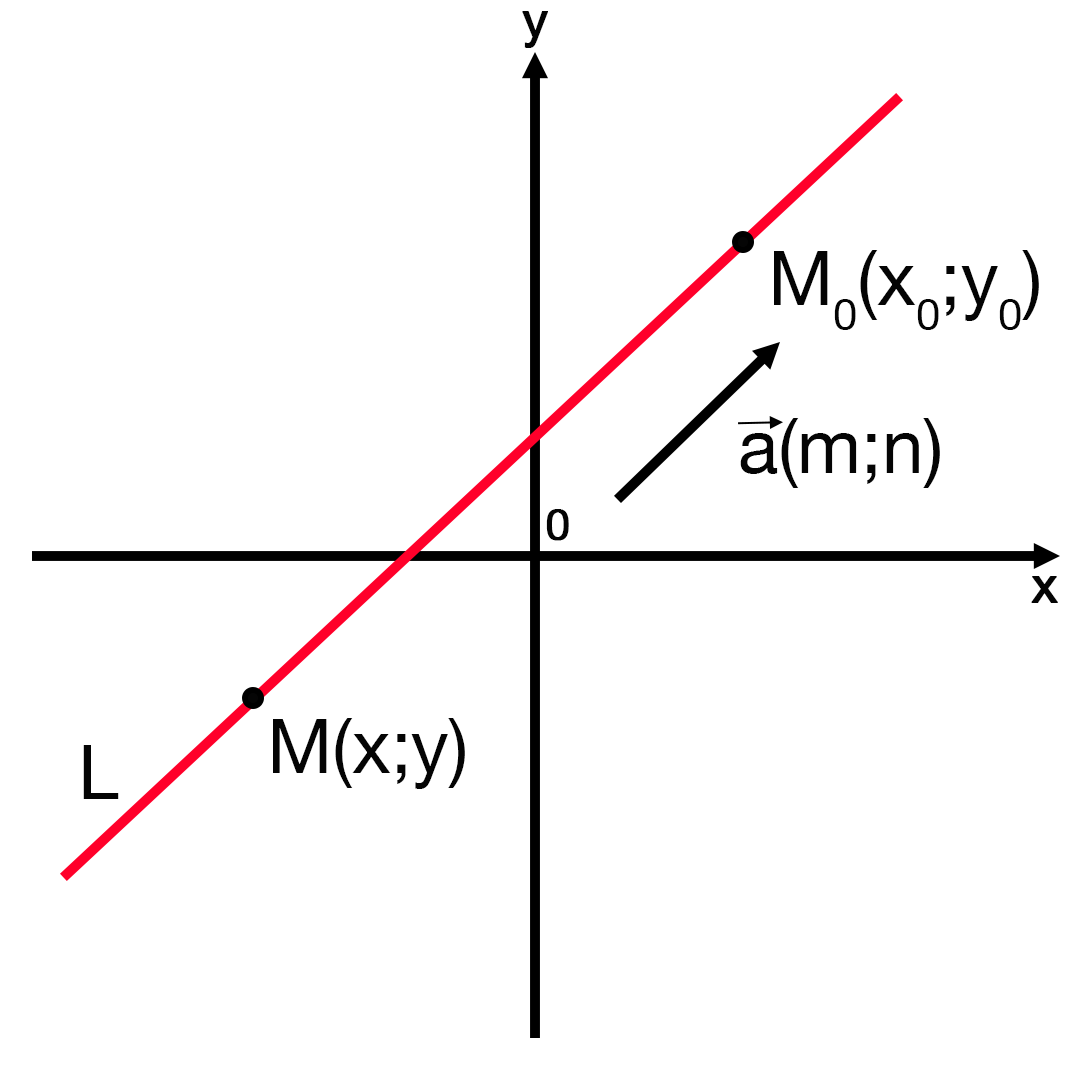
\includegraphics[width=0.5\textwidth]{kanon_line.png}
\end{center}

Условием коллинеарности векторов \(\overrightarrow{M_0M}\) и \(\overrightarrow{a}\) будет:
\(\dfrac{x - x_0}{m} = \dfrac{y - y_0}{n}\), что и является каноническим уравнением прямой.

\subsection*{Уравнение прямой через 2 заданные точки}

Даны две точки \(M_0(x_0;y_0)\) и \(M_1(x_1;y_1)\), лежащие на прямой \(L\).
Из этого следует, что \(\overrightarrow{M_0M_1} = (x_1 - x_0; y_1 - y_0)\) — направляющий вектор прямой \(L\).

Тогда искомое уравнение будет иметь вид: \(\dfrac{x - x_0}{x_1 - x_0} = \dfrac{y - y_0}{y_1 - y_0}\).

\subsection*{Параметрическое уравнение прямой}

Уравнение \(\overrightarrow{M_0M} = \lambda \cdot \overrightarrow{a}\) называют векторно-параметрическим уравнением прямой, где \lambda — некоторое действительное число.

В векторной форме оно имеет вид:
\begin{align*}
     &  &
    \overrightarrow{M_0M} = \lambda \cdot \overrightarrow{a} \iff
    \begin{cases}
        x - x_0 = \lambda \cdot m \\
        y - y_0 = \lambda \cdot n
    \end{cases}
    \iff
    \begin{cases}
        x = x_0 + \lambda \cdot m \\
        y = y_0 + \lambda \cdot n
    \end{cases}
\end{align*}

\subsection*{Общее уравнение прямой}

Уравнение, имеющее вид \(Ax + By + C = 0 \) — это общее уравнение прямой на плоскости в прямоугольной системе координат \(Oxy\).

\subsubsection*{Теорема}
Любое уравнение первой степени, имеющее вид \(Ax + By + C = 0\), где \(A, B, C\) – некоторые действительные числа (\(A\) и \(B\) не равны одновременно нулю) определяет прямую линию в прямоугольной системе координат на плоскости.
В свою очередь, любая прямая в прямоугольной системе координат на плоскости определяется уравнением, имеющим вид \(Ax + By + C = 0\) при некотором наборе значений \(A, B, C\).
\subsubsection*{Доказательство}
Теорема состоит из 2-х пунктов. Докажем каждый из них: \\

\textbf{Пункт 1}. Уравнение \(Ax + By + C = 0\) определяет на плоскости прямую. \\

Пусть существует некоторая точка М 0 ( x 0 ,   y 0 ) М0(x0, y0), координаты которой отвечают уравнению \(Ax + By + C = 0\). Таким образом: \(Ax_0 + By_0 + C = 0\).
Вычтем из левой и правой частей уравнений \(Ax + By + C = 0\) левую и правую части уравнения \(Ax_0 + By_0 + C = 0\), получим новое уравнение, имеющее вид \(A(x - x_0) + B(y - y_0) + C = 0\).
Оно эквивалентно \(Ax + By + C = 0\).

Полученное уравнение \(A(x - x_0) + B(y - y_0) + C = 0\) является необходимым и достаточным условием перпендикулярности векторов \(\overrightarrow{n} = (A, B)\) и \(\overrightarrow{M_0M} = (x - x_0, y - y_0)\).
Таким образом множество точек \(M(x, y)\) задает в прямоугольной системе координат прямую линию, перпендикулярную направлению вектора \(\overrightarrow{n} = (A, B)\).

Предположим, что это не так. Тогда вектор \(\overrightarrow{n} = (A, B)\) не перпендикулярен вектору \(\overrightarrow{M_0M} = (x - x_0, y - y_0)\), а равенство \(A(x - x_0) + B(y - y_0) = 0\) не является верным.

\begin{center}
    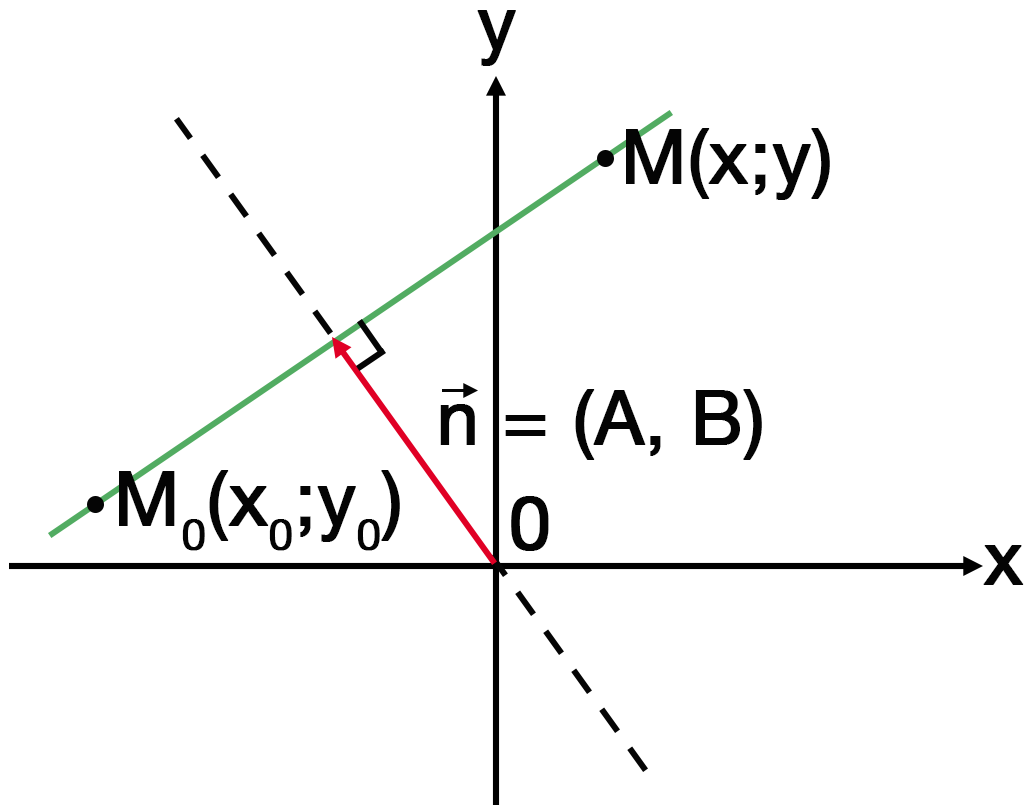
\includegraphics[width=0.5\textwidth]{general_line.png}
\end{center}

Следовательно, уравнение \(A(x - x_0) + B(y - y_0) = 0\) определяет некоторую прямую в прямоугольной системе координат на плоскости, а значит и эквивалентное ему уравнение \(Ax + By + C = 0\) определяет ту же прямую. \\

\textbf{Пункт 2}. Любую прямую в прямоугольной системе координат на плоскости можно задать уравнением первой степени \(Ax + By + C = 0\). \\

Зададим в прямоугольной системе координат на плоскости прямую \(a \); точку \(M_0(x_0, y_0)\), через которую проходит эта прямая, а также нормальный вектор этой прямой \(\overrightarrow{n} = (A, B)\).
Пусть точка \(M(x, y)\) — произвольная точка на прямой, тогда векторы \(\overrightarrow{n} = (A, B)\) и \(\overrightarrow{M_0M} = (x - x_0, y - y_0)\) являются перпендикулярными друг другу и их скалярное произведение равно нулю:
\begin{align*}
     &  &
    (\overrightarrow{n}, \overrightarrow{M_0M}) = A(x - x_0) + B(y - y_0) = 0
\end{align*}

Пусть \(C = -Ax_0 - By_0\), тогда получим уравнение:
\begin{align*}
     &  &
    Ax + By + C = 0
\end{align*}



\newpage

\section{Парабола. Определение, вывод уравнения, характеристики}\label{sec:parabola}

\subsection*{Определение}
Парабола — геометрическое место точек на плоскости, равноудалённых от данной прямой \(d\) и данной точки \(F\).
Точка \(F\) не лежит ни на кривой, ни на прямой \(d\).

Точка \(F\) называется \textbf{фокусом}, а прямая \(d\) — \textbf{директрисой параболы}.
Расстояние от фокуса до директрисы называется \textbf{фокальным параметром} параболы и обозначается через \(p\).

\textbf{Эксцентриситет} параболы — это отношение расстояний от произвольной точки на кривой до фокуса и от этой же точки до директрисы.
Эксцентриситет параболы по определению равен 1.

Каноническое уравнение параболы: \(y^2 = 2px\)

\subsection*{Вывод канонического уравнения}

Пусть фокус \(F\) принадлежит оси \(OX\).
Проведем директрису перпендикулярно оси \(OX\) на расстоянии \(p\) от фокуса \(F\), тогда пусть т. \(O\) будет серединой этого расстояния.
Возьмем т. \(M(x; y)\), которая принадлежит параболе.
Расстояние от т. \(M(x; y)\) до фокуса обозначим за \(r\), до директрисы за \(d\).

\begin{center}
    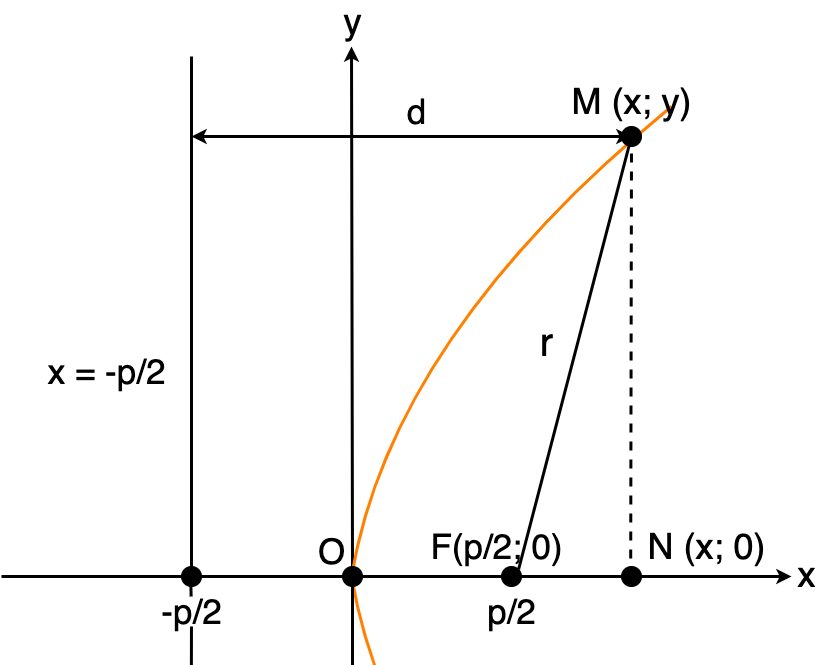
\includegraphics[width=0.8\textwidth]{parabola.png}
\end{center}

Расстояние от т. \(M(x;y)\) до директрисы равно \(d = \Big| x + \dfrac{p}{2} \Big| \).

По определению параболы \(r = d\).

По теореме Пифагора из прямоугольного \(\Delta FMN\): \(r=\sqrt{\Big(x - \dfrac{p}{2}\Big)^2 + y^2}\)

Следовательно:

\begin{gather*}
    \sqrt{\Big(x - \frac{p}{2}\Big)^2 + y^2} = x + \frac{p}{2} \\
    x^2 - px + \frac{p^2}{4} + y^2 = x^2 + px + \frac{p^2}{4} \\
    y^2 = 2px
\end{gather*}

\subsection*{Свойства параболы}

\begin{itemize}
    \item[—]{Имеет ось симметрии называемой осью параболы. Ось проходит через фокус и вершину перпендикулярно директрисе;}
    \item[—]{Если фокус параболы отразить относительно касательной, то его образ будет лежать на директрисе;}
    \item[—]{Все параболы подобны. Расстояние между фокусом и директрисой определяет масштаб;}
\end{itemize}

\end{document}
